\subsection{Нечетная функция}

Рассмотрим нечетную периодическую функцию с периодом $T = \pi$:

\begin{equation}
    f_3(t) = |\cos(2t) \cdot \sin(t)|
\end{equation}

График этой функции приведен на рис.~\ref{fig:func_3}.

\begin{figure}[ht!]
    \centering
    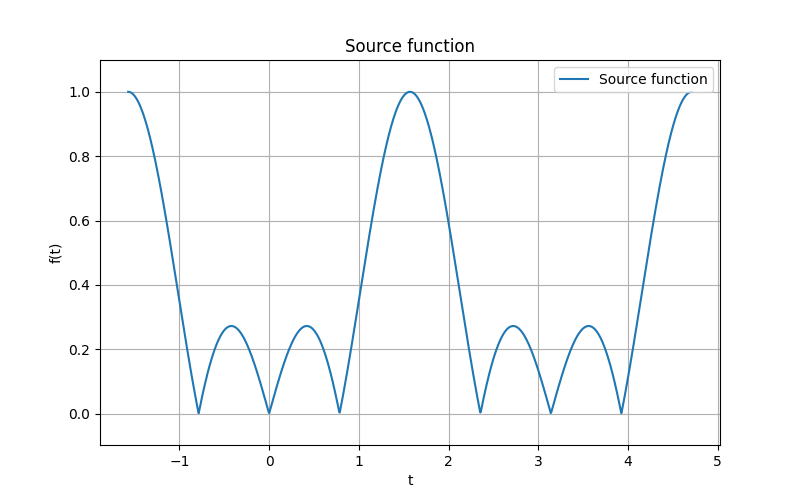
\includegraphics[width=\textwidth]{media/plots/func_3.png}
    \caption{График функции $f_3(t)$}
    \label{fig:func_3}
\end{figure}

\subsubsection{Вычисление коэффициентов Фурье}
Найдем коэффициенты ряда Фурье для этой функции:

\begin{equation}
    a_n = \frac{2}{\pi}\int\limits_{0}^{\pi} |\cos(2t) \cdot \sin(t)| \cos(2nt) dt 
\end{equation}

\begin{equation}
    b_n = \frac{2}{\pi}\int\limits_{0}^{\pi} |\cos(2t) \cdot \sin(t)| \sin(2nt) dt 
\end{equation}

\begin{equation}
    c_n = \frac{1}{\pi}\int\limits_{0}^{\pi} |\cos(2t) \cdot \sin(t)| e^{-2int} dt 
\end{equation}


\subsubsection{Вычисление коэффициентов Фурье с помощью программы}

\begin{lstlisting}[style=python_white, caption=Вычисление коэффициентов Фурье, label=lst:func_3]
func = np.vectorize(lambda x: abs(np.cos(2 * x) * np.sin(x)))
a, b = fourier(func, 0, np.pi, 3)
print_fourier_coefficients(a, b)
c = fourier_exp(func, 0, np.pi, 3)
print_fourier_exp_coefficients(c)
\end{lstlisting}

В результате выполнения программы (\ref{lst:func_3}) получим следующие значения (см. таблицу~\ref{tab:func_3}~и~\ref{tab:func_3_exp}).

% table with coefficients
\begin{table}[ht!]
    \centering
    \begin{tabular}{|c|c|c|}
        \hline
        $n$ & $a_n$ & $b_n$ \\
        \hline
        0 & 0.77601 & 0.0 \\
        1 & -0.36616 & 0.0 \\
        2 & 0.21548 & 0.0 \\
        3 & -0.09828 & 0.0 \\
        \hline
    \end{tabular}
    \caption{Коэффициенты Фурье для функции $f_3(t)$}
    \label{tab:func_3}
\end{table}

\begin{table}[ht!]
    \centering
    \begin{tabular}{|c|c|}
        \hline
        $n$ & $c_n$ \\
        \hline
        -3 & -0.04914 \\
        -2 & 0.10774 \\
        -1 & -0.18308 \\
        0 & 0.38800 \\
        1 & -0.18308 \\
        2 & 0.10774 \\
        3 & -0.04914 \\
        \hline
    \end{tabular}
    \caption{Коэффициенты Фурье для функции $f_3(t)$ (комплексный случай)}
    \label{tab:func_3_exp}
\end{table}

\subsubsection{Построение графиков частичных сумм ряда Фурье}
В качество значений $N$ выберем $N = 1, 2, 3, 4, 5$. Для каждого значения $N$ вычислим частичную сумму ряда Фурье и построим график (см. рис.~\ref{fig:func_3_plot}~и~\ref{fig:func_3_plot_exp}).

\begin{lstlisting}[style=python_white, caption=Построение графиков частичных сумм ряда Фурье, label=lst:func_1_plot]
func = np.vectorize(lambda x: abs(np.cos(2 * x) * np.sin(x)))
calc_and_plot(func, 0, np.pi, [1, 2, 3, 4, 5], './media/plots/func_3')
calc_and_plot_exp(func, 0, np.pi, [1, 2, 3, 4, 5], './media/plots/func_3_exp')
\end{lstlisting}

% plot with partial sums
\begin{figure}[ht!]
    \centering
    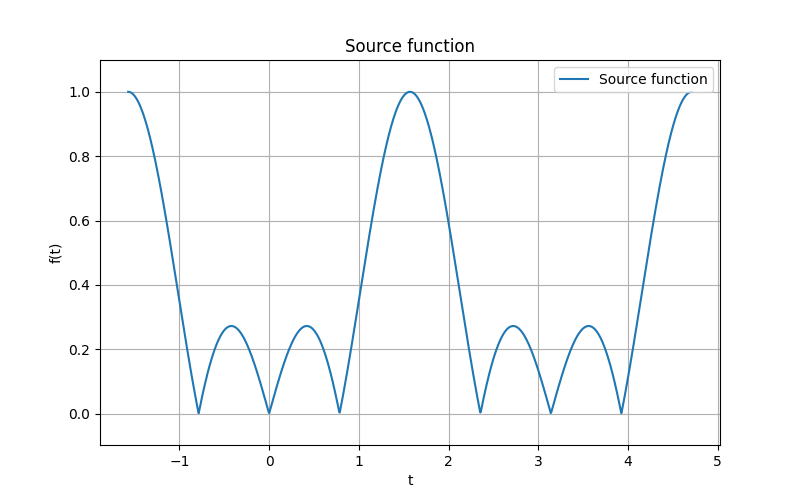
\includegraphics[width=0.49\textwidth]{media/plots/func_3_exp.png}
    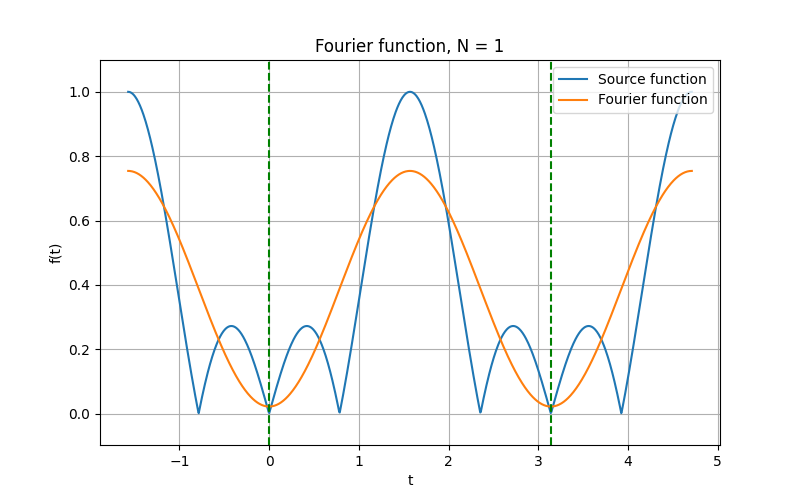
\includegraphics[width=0.49\textwidth]{media/plots/func_3_N_1.png}
    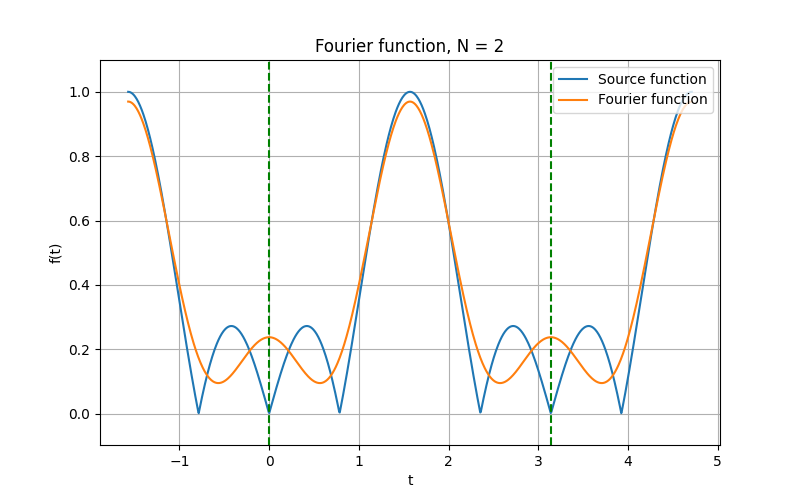
\includegraphics[width=0.49\textwidth]{media/plots/func_3_N_2.png}
    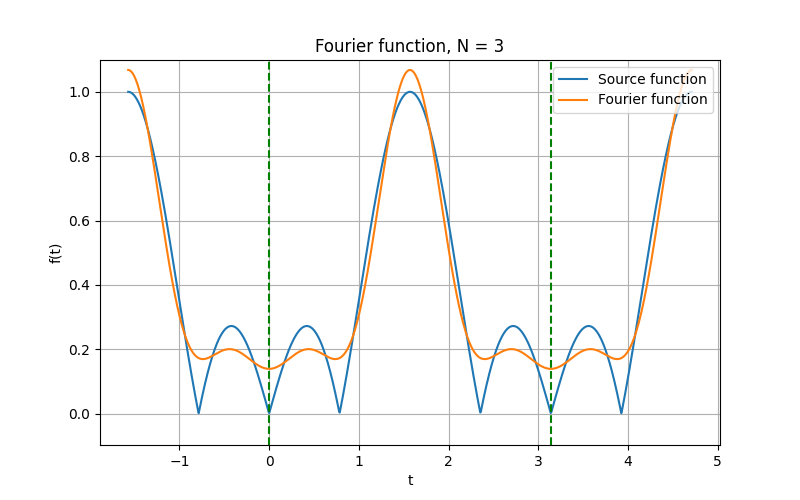
\includegraphics[width=0.49\textwidth]{media/plots/func_3_N_3.png}
    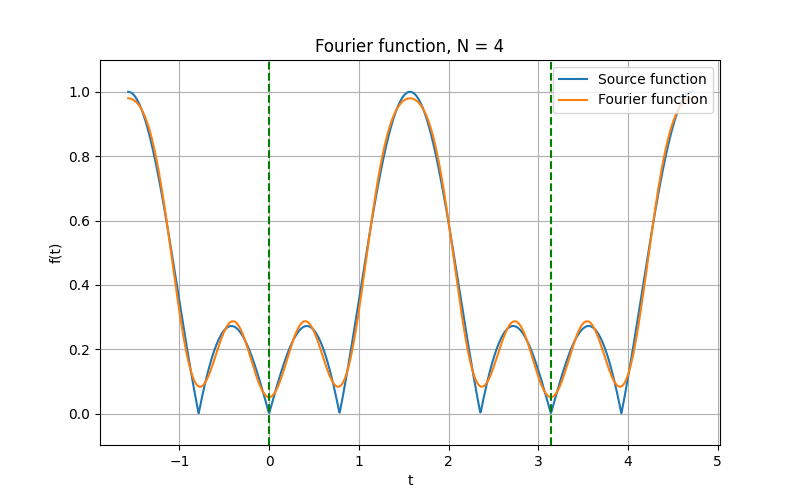
\includegraphics[width=0.49\textwidth]{media/plots/func_3_N_4.png}
    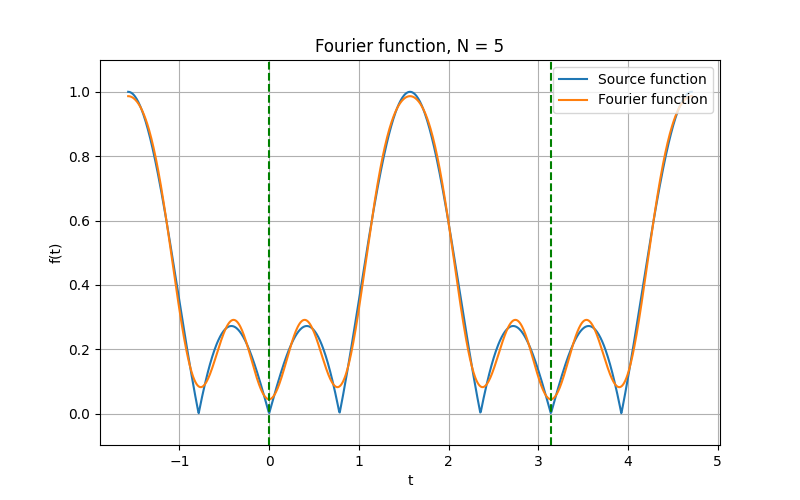
\includegraphics[width=0.49\textwidth]{media/plots/func_3_N_5.png}
    \caption{График частичных сумм ряда Фурье для функции $f_3(t)$}
    \label{fig:func_3_plot}
\end{figure}

\begin{figure}[ht!]
    \centering
    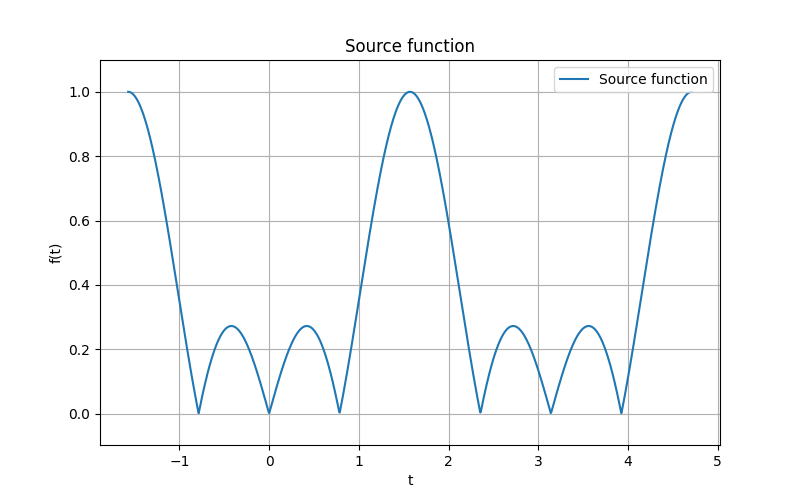
\includegraphics[width=0.49\textwidth]{media/plots/func_3.png}
    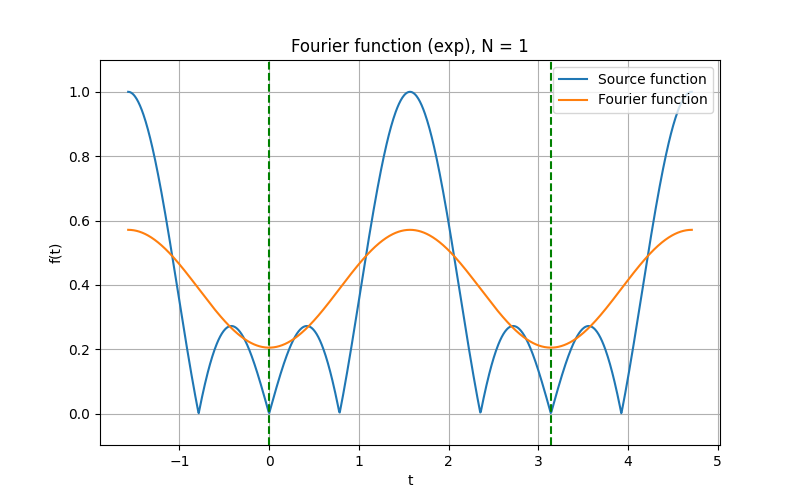
\includegraphics[width=0.49\textwidth]{media/plots/func_3_exp_N_1.png}
    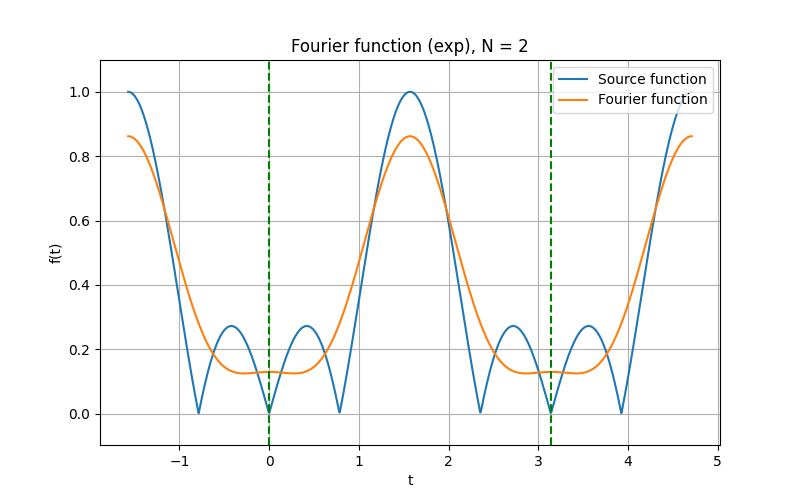
\includegraphics[width=0.49\textwidth]{media/plots/func_3_exp_N_2.png}
    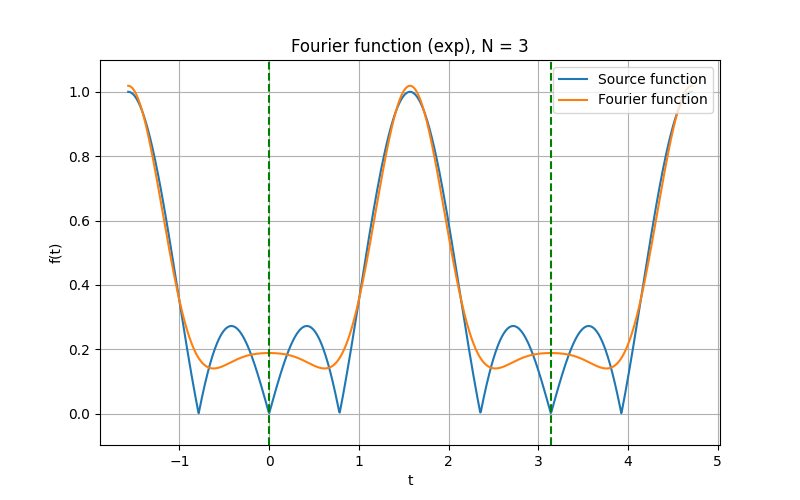
\includegraphics[width=0.49\textwidth]{media/plots/func_3_exp_N_3.png}
    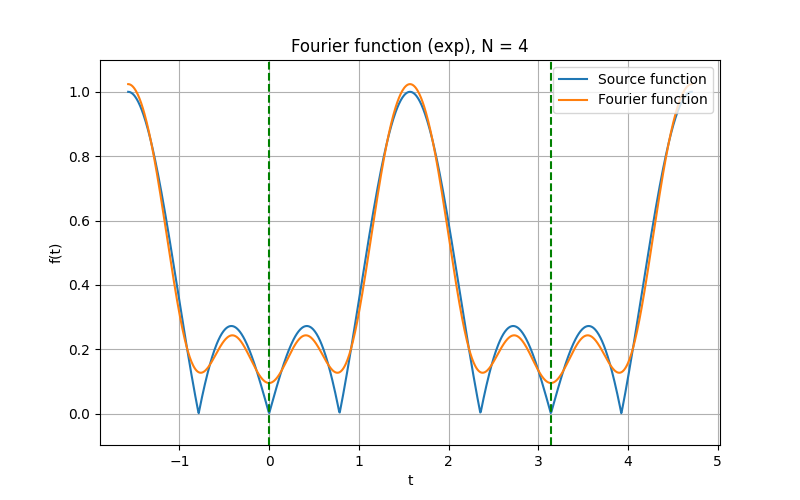
\includegraphics[width=0.49\textwidth]{media/plots/func_3_exp_N_4.png}
    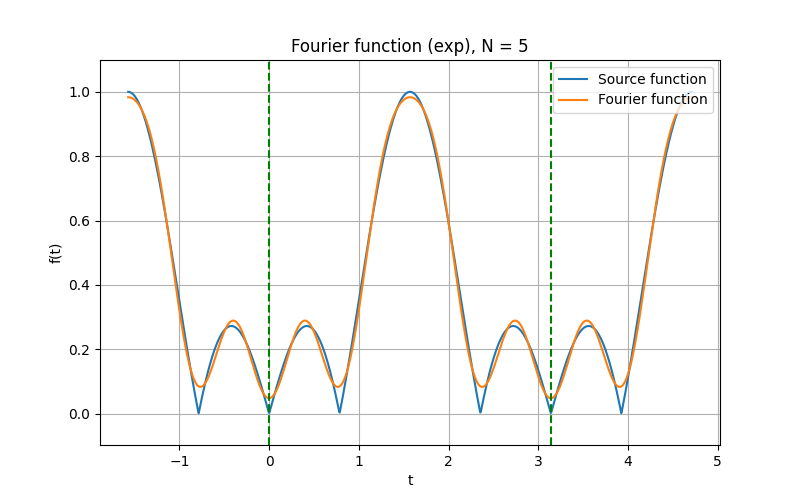
\includegraphics[width=0.49\textwidth]{media/plots/func_3_exp_N_5.png}
    \caption{График частичных сумм ряда Фурье для функции $f_3(t)$}
    \label{fig:func_3_plot_exp}
\end{figure}


Видим, что при увеличении $N$ график частичной суммы ряда Фурье приближается к исходной функции, но, в отличие от четной функции, не становится неотличимым от исходной функции при $N = 5$.

\FloatBarrier
\subsubsection{Проверка равенства Парсеваля}

Проверим равенство Парсеваля для функции $f_3(t)$:

Для этого воспользуемся функцией \texttt{perseval\_check} (см. листинг~\ref{lst:perseval_check}).
Мною была рассмотрена сумма трехсот коэффициентов. Этого оказалось достаточно для равенства квадрата нормы и суммы до 6 знака. 

\begin{table}[ht!]
    \centering
    \begin{tabular}{|c|c|c|}
        \hline
        $||f_3||^2$ & $2\pi \sum\limits_{n = -\infty}^{300} |c_n|^2$ & $\pi \left(\frac{a_0^2}{2} + \sum\limits_{n = 1}^{300} (a_n^2 + b_n^2)\right)$\\
        \hline
        1.57080 & 1.57080 & 1.57080 \\
        \hline
    \end{tabular}
    \caption{Проверка равенства Персеваля для функции $f_3(t)$}
    \label{tab:func_3_pers}
\end{table}